%%%%%%%%%%%%%%%%%%%%%%%%%%%%%%%%%%%%%%%%%

\chapter{UCN spin manipulation}\label{chap:spinManipulation}

%%%%%%%%%%%%%%%%%%%%%%%%%%%%%%%%%%%%%%%%%

This chapter introduces the spin manipulation techniques used in the \acrshort*{lanl} \acrshort*{nedm} experiment. Sections \ref{sec:larmor} -- \ref{sec:ramsey-method} discuss the main magnetic resonance techniques in the \acrshort*{lanl} \acrshort*{nedm} experiment. This includes Ramsey method of separated oscillatory fields, which is used for the measurement of the spin precession frequency of stored \ucn in a static magnetic field.   Section~\ref{sec:bloch_equations} is about the Bloch equations, which describes \ucn spin interactions in the semiclassical regime, and are often used in \ucn spin tracking simulations.

Nuclear magnetic resonance (\acrshort*{nmr}) was first observed by Rabi in 1938 \cite{rabi_1938}, where he utilized a Stern-Gerlach experiment with a beam of nuclei traversing an inhomogenous magnetic field. He introduced an additional \acrshort{rf} magnetic field perpendicular to the static field. When the strength of the static field was tuned properly, there was a dip in beam intensity at the detector. This dip corresponded to a transition in the spin state of the nuclei, with the minimum at the resonance condition where the Larmor precession frequency of the nuclei in the static field matched the frequency of the \acrshort*{rf} field. Sweeping the strength of the static field to find the resonance enabled Rabi to measure the nuclear magnetic moment. Section~\ref{sec:rabi} describes the Rabi method in more detail, examining the more typical experimental application methodology where \acrshort{rf} frequency is swept and the static field is held constant to find resonance.

In 1949, Ramsey improved upon the Rabi method \cite{ramsey_molecular_1950}.  He divided the single oscillatory magnetic field at the center of the Rabi device into two shorter ones, one at the beginning of the beam and one at the end. This offers a number of advantages, the main one being that the peak near resonance is narrower than from the Rabi method, giving higher resolution for determining the resonant frequency. The narrowing is analogous to the peaks in a double slit diffraction experiment, which are narrower than the peak from a single slit of equal width to the separation of the double slits \cite{Ekspong1993}.

Of course, even the most advanced NMR techniques are ineffective if neutrons are not effectively polarized and if the polarization cannot be maintained. Section~\ref{sec:ucn_polarizers} discusses neutron polarization methodology and Sec.~\ref{sec:spin_relaxation} covers spin coherence. Section~\ref{sec:adiabaticity} introduces the adiabaticity parameter commonly used to characterize the conditions of neutron spin transport. Section~\ref{sec:afp} discusses the mechanics of the adiabatic fast passage spin flipper that is located before the spin analyzer and neutron detector (see \comment{AFP description section}).

%%%%%%%%%%%%%%%%%%%%%%%%%%%%%%%%%%%%%%%%%

\section{UCN polarizers}\label{sec:ucn_polarizers}

%%%%%%%%%%%%%%%%%%%%%%%%%%%%%%%%%%%%%%%%%

\ucn must first be polarized before being subjected to spin manipulation techniques. There are two main methods for \ucn polarization: \comment{(1)... (2)}

%%%%%%%%%%%%%%%%%%%%%%%%%%%%%%%%%%%%%%%%%

\section{Precession in a uniform static magnetic field\label{sec:larmor}}

%%%%%%%%%%%%%%%%%%%%%%%%%%%%%%%%%%%%%%%%%

We begin with the classic undergraduate example of precession in a static field \cite{griffiths_quantum}. The Hamiltonian operator for a magnetic dipole moment in a magnetic field \gls*{bField} is
%
\begin{align}
    \hat{H}=-\hat{\mu}\cdot\gls*{bField}=-\gamma\hat{S}\cdot \gls*{bField}\label{eq:hamiltonian_operator}
\end{align}
%
for magnetic dipole moment operator $\hat{\mu}$, gyromagnetic ratio $\gamma$, and spin operator $\hat{S}=\frac{\hbar}{2}\vv{\sigma}$. Let \gls*{bField} be a static magnetic field such that $\gls*{bField}=B_0 \vv{z}$. Therefore,
%
\begin{gather}
    \hat{H}=-\gamma B_0 \hat{S}_z=-\frac{\gamma \hbar B_0}{2}\sigma_z\label{eq:larmor_1}
\end{gather}
%
The Pauli matrices, written as $\vv{\sigma}=(\sigma_x, \sigma_y, \sigma_z)$, are
%
\begin{gather}
    \sigma_{x}=\left(\begin{matrix}
    0 & 1\\
    1 & 0
    \end{matrix}\right)\quad
    \sigma_{y}=\left(\begin{matrix}
    0 & -i\\
    i & 0
    \end{matrix}\right)\quad
    \sigma_{z}=\left(\begin{matrix}
    1 & 0\\
    0 & -1
    \end{matrix}\right)
\end{gather}
%
The time dependent \schrodinger equation is
%
\begin{gather}
    i\hbar\frac{d}{dt}\Ket{\psi(t)}=\hat{H}\Ket{\psi(t)} \label{eq:schrodinger}
\end{gather}
%
where we write the spinor as 
\begin{gather}
    \Ket{\psi(t)}=\Ket{\begin{matrix}
        \psi_+(t)\\
        \psi_-(t)
    \end{matrix}}\label{eq:spinor}  
\end{gather}
%
Substituting (\ref{eq:larmor_1}) into (\ref{eq:schrodinger}),
\begin{gather}
    \left(\begin{matrix}
        \dot{\psi}_+\\
        \dot{\psi}_-
    \end{matrix}\right)
    = -\frac{i\omega_0}{2}
    \left(\begin{matrix}
        1 & 0\\
        0 & -1
    \end{matrix} \right)
    \left(\begin{matrix}
        \psi_+\\
        \psi_-
    \end{matrix}\right)\label{eq:larmor_2}
\end{gather}
where we define the Larmor precession frequency as
%
\begin{gather}
    \omega_0 = -\gamma B_0 \label{eq:larmor_freq}
\end{gather}
%
Eq.~(\ref{eq:larmor_2}) simplifies into the differential equations
%
\begin{align}
    \dot{\psi}_+ &=\frac{-i\omega_0}{2}\psi_+ \label{eq:larmor_3}\\
    \dot{\psi}_- &=\frac{i\omega_0}{2}\psi_- \label{eq:larmor_4}
\end{align}
%
Let the initial condition at $t=0$ be 
$\Ket{\psi(t=0)}=\left( \begin{matrix}
    a_0 \\
    b_0
\end{matrix}\right)$. Solving Eqs.~(\ref{eq:larmor_3}) and (\ref{eq:larmor_4}) gives the solution
%
\begin{gather}
    \ket{\psi(t)}=\left(\begin{matrix}
        a_0e^{-i\omega_0 t/2} \\
        b_0e^{i\omega_0 t/2}
    \end{matrix}\right)\label{eq:larmor_solution}
\end{gather}
%
where $a_0$ and $b_0$ can be complex numbers. To obtain the odds of measuring spin up along $x$, $y$, and $z$, we use the normalized eigenvectors of the Pauli matrices
%
\begin{gather}
    \Ket{S_z;+}=\left(\begin{matrix}
        1 \\
        0
    \end{matrix}\right),\quad
    \Ket{S_y;+}=\frac{1}{\sqrt{2}}\left(\begin{matrix}
        1 \\
        i
    \end{matrix}\right),\quad
    \Ket{S_x;+}=\frac{1}{\sqrt{2}}\left(\begin{matrix}
        1 \\
        1
    \end{matrix}\right)\label{eq:pauli_eigenvectors}
\end{gather}
%
Therefore,
%
\begin{align}
    \left| \Braket{S_z;+ | \psi(t)} \right|^2&= |a_0|^2 \\
    \left| \Braket{S_x;+ | \psi(t)} \right|^2&= \frac{1}{2} + \frac{1}{2}(a_0b_0^*+a_0^*b_0)\cos\,\omega_0t - \frac{1}{2}i(a_0b_0^*-a_0^*b_0)\sin\,\omega_0t \label{eq:larmor_5} \\
    \left| \Braket{S_y;+ | \psi(t)} \right|^2&= \frac{1}{2} + \frac{1}{2}i(a_0^*b_0-a_0b_0^*)\cos\,\omega_0t - \frac{1}{2}(a_0b_0^*+a_0^*b_0)\sin\,\omega_0t \label{eq:larmor_6}
\end{align}
%
This corresponds to the particle precessing about $\vv{z}$ at the Larmor frequency $\omega_0$. For example, for an initial state $a_0=1/\sqrt{2}, b_0=1/\sqrt{2}$ (where the semiclassical spin vector points along $\vv{x}$ in the $x \text{ -- } y$ plane), Eqs.~(\ref{eq:larmor_5}) and (\ref{eq:larmor_6}) become
%
\begin{align}
    \left| \Braket{S_x;+ | \psi(t)} \right|^2&= \frac{1}{2} + \frac{1}{2}\cos\,\omega_0t \\
    \left| \Braket{S_y;+ | \psi(t)} \right|^2&= \frac{1}{2} - \frac{1}{2}\sin\,\omega_0t 
\end{align}

%%%%%%%%%%%%%%%%%%%%%%%%%%%%%%%%%%%%%%%%%

\section{Rabi resonance\label{sec:rabi}}

%%%%%%%%%%%%%%%%%%%%%%%%%%%%%%%%%%%%%%%%%

We now consider the case with a field $\vv{B_\text{c}}$ (which we will refer to as a ``circular \acrshort{rf}'') rotating at a frequency $\omega$ in the $x$ -- $y$ plane with an initial phase $\phi$ relative to $x$. The total field $\vv{B}$ becomes
%
\begin{gather}
    \vv{B}(t)=\vv{B_\text{c}}(t) + \vv{B_0}=B_\text{c}\left[ \cos (\omega t + \phi) \vv{x} + \sin (\omega t + \phi) \vv{y}\right] + B_0 \vv{z}
\end{gather}
%
with the condition that $B_\text{c} \ll B_0$. The Hamiltonian operator from Eq.~\ref{eq:hamiltonian_operator} becomes
%
\begin{gather}
    \hat{H} = -\gamma \left( B_\text{c} \hat{S}_x \cos (\omega t + \phi) + B_\text{c} \hat{S}_y  \sin (\omega t + \phi) + B_0\hat{S}_z \right)\label{eq:rabi_hamiltonian}
\end{gather}
%
We define the resonant angular frequency for the circular \acrshort*{rf} as $\omega_\text{c}=-\gamma B_\text{c}$. Using the \schrodinger equation (\ref{eq:schrodinger}) and (\ref{eq:spinor}), this gives
%
\begin{gather}
    \left(\begin{matrix}
        \dot{\psi}_+\\
        \dot{\psi}_-
    \end{matrix}\right)
    = -\frac{i}{2}
    \left(\begin{matrix}
        \omega_0 & \omega_\text{c}e^{-i(\omega t + \phi)}\\
        \omega_\text{c}e^{i(\omega t + \phi)} & -\omega_0
    \end{matrix} \right)
    \left(\begin{matrix}
        \psi_+\\
        \psi_-
    \end{matrix}\right)\label{eq:rabi_1}
\end{gather}
%
where $\omega_0$ is the Larmor frequency (\ref{eq:larmor_freq}). We rewrite Eq.~\ref{eq:rabi_1} as
%
\begin{align}
    \dot{\psi}_+ &=\frac{-i}{2}\left( \omega_0 \psi_+ + \omega_\text{c} e^{-i(\omega t + \phi)} \psi_- \right)\label{eq:rabi_2}\\
    \dot{\psi}_- &=\frac{i}{2}\left( \omega_0 \psi_- - \omega_\text{c} e^{i(\omega t + \phi)} \psi_+ \right)\label{eq:rabi_3}
\end{align}
%
To solve these differential equations, we make the change of variables $\psi_+ = \psi'_+ e^{-i(\omega t + \phi)/2}$ and $\psi_- = \psi'_- e^{i(\omega t + \phi)/2}$, which gives
%
\begin{align}
    \dot{\psi}'_+ &= \frac{i}{2}((\omega - \omega_0)\psi'_+ - \omega_\text{c} \psi'_-)\label{eq:rabi_4}  \\
    \dot{\psi}'_- &= -\frac{i}{2}(\omega_\text{c}\psi'_+ + (\omega - \omega_0) \psi'_-)\label{eq:rabi_5} 
\end{align}
%
We then decouple by taking another derivative of (\ref{eq:rabi_4}) and (\ref{eq:rabi_5}) with respect to $t$ and use some algebra to get
%
\begin{gather}
     \ddot{\psi'}_{\pm} = -\Omega^2 \psi'_{\pm}\label{eq:rabi_6}
\end{gather}
%
where we let the Rabi flopping frequency be 
%
\begin{gather}
   \Omega=\frac{\sqrt{(\omega - \omega_0)^2+\omega_\text{c}^2}} {2}  \label{eq:rabi_freq}
\end{gather}
%
The solution for (\ref{eq:rabi_6}) has the form
%
\begin{gather}
    \psi'_\pm= C_{\psi\pm}\cos\,\Omega t + D_{\psi\pm}\sin\,\Omega t
\end{gather}
%
which in the original basis is
%
\begin{gather}
    \psi_\pm= e^{\mp i (\omega t+\phi)/2}\left( C_{\psi\pm}\cos\,\Omega t + D_{\psi\pm}\sin\,\Omega t \right)
\end{gather}
%
Solving initial conditions (see Ref.~\cite{may_thesis}) for
$\Ket{\psi(t=0)}=\left( \begin{matrix}
    a_0 \\
    b_0
\end{matrix}\right)$, where $a_0$ and $b_0$ are complex, gives
%
\begin{align}
    \psi_+(t) &= e^{-i(\omega t + \phi)/2}\left(a_0 e^{i\phi/2} \cos \, \Omega t + D_{\psi +} \sin \, \Omega t\right) \\
    \psi_-(t) &= e^{i(\omega t + \phi)/2}\left(b_0 e^{-i\phi/2} \cos \, \Omega t + D_{\psi -} \sin \, \Omega t\right) \\
    D_{\psi +} &= \frac{i}{2\Omega}\left( a_0 e^{i\phi/2} (\omega - \omega_0) - \omega_\text{c}b_0 e^{-i\phi/2} \right) \\
    D_{\psi -} &= -\frac{i}{2\Omega} \left(a_0 \omega_\text{c}e^{i\phi/2} + b_0(\omega -\omega_0)e^{-i\phi/2} \right)
\end{align}
%
As before, the probability of measuring spin up along $x$, $y$, and $z$ are determined by using (\ref{eq:pauli_eigenvectors})
%
\begin{align}
    \left| \Braket{S_z;+ | \psi(t)} \right|^2&= \psi_+(t)\psi_+^*(t) \\
    \left| \Braket{S_x;+ | \psi(t)} \right|^2&= \frac{1}{2} + \frac{1}{2}( \psi_+(t)\psi_-^*(t)) \\
    \left| \Braket{S_y;+ | \psi(t)} \right|^2&= \frac{1}{2} + \frac{i}{2}( \psi_-(t)\psi_+^*(t) - \psi_+(t)\psi_-^*(t) )
\end{align}
%
Let us consider the instance where the particle starts spin up along $z$ where $\psi_+(t=0)=a_0=1$ and $\psi_-(t=0)=b_0=0$. This reproduces Rabi's result \cite{rabi_1938} where
%
\begin{gather}
    \left| \Braket{S_z;+ | \psi(t)} \right|^2 = 1-\left( \frac{\omega_\text{c}}{(\omega -\omega_0)^2+\omega_\text{c}^2} \right) \sin^2\Omega t \label{eq:rabi_7}
\end{gather}
%
\comment{describe more qualitative behavior in the semi classical limit with more plots}

At the resonance condition, $\omega=\omega_0$ and $\left| \Braket{S_z;+ | \psi(t)} \right|^2=0$. Equation~(\ref{eq:rabi_7}) simplifies into the expression
%
\begin{gather}
    \omega_\text{c}=\frac{(2n-1)\pi}{t}
\end{gather}
%
The integer $n$ describes how many spin flips the neutron undergoes while the \acrshort*{rf} is applied for a duration $t$. A single spin flip from the Rabi method is often referred to as a ``$\pi$ flip,'' and an on-resonance application of the \acrshort*{rf} field induce the $\pi$ flip is called a ``$\pi$ pulse.''

%%%%%%%%%%%%%%%%%%%%%%%%%%%%%%%%%%%%%%%%%

\subsection{Rabi resonance with a linear RF field}

%%%%%%%%%%%%%%%%%%%%%%%%%%%%%%%%%%%%%%%%%

In an experimental setting it is more practical to generate a linear \acrshort*{rf} field. For a linear \acrshort*{rf} field $\vv{B_\ell}$ under the condition $B_\ell \ll B_0$, the magnetic field is now written as
%
\begin{gather}
    \vv{B}(t)=\vv{B_\ell}(t) + \vv{B_0}=B_\ell \cos (\omega t + \phi) \vv{x} + B_0 \vv{z}
\end{gather}
%
We again let the frequency be $\omega_\ell=-\gamma B_\ell$. Following the procedure in Sec.~\ref{sec:rabi}, we use the \schrodinger equation to get
%
\begin{align}
    \dot{\psi}_+ &=\frac{-i}{2}\left( \omega_0 \psi_+ + \omega_\ell \psi_-  \cos(\omega t + \phi) \right)\label{eq:rabi_linear_1}\\
    \dot{\psi}_- &=\frac{i}{2}\left( \omega_0 \psi_- - \omega_\ell \psi_+ \cos(\omega t + \phi)  \right)\label{eq:rabi_linear_2}
\end{align}
%
This is solved numerically, as described in Appx.~\ref{appx:ramsey_numerical}. \comment{Todo: insert images of linear RF flips}

As per Ref.~\cite{rabi_1938}, Rabi flips from a linear \acrshort*{rf} behave similarly to the result from  Sec.~\ref{sec:rabi} by the substitution $\omega_\ell/2\approx\omega_\text{c}$ with an additional caveat. Section~\ref{sec:bloch-siegert} further describes this distinction between circular and linear \acrshort*{rf} $\pi$ flips.


%%%%%%%%%%%%%%%%%%%%%%%%%%%%%%%%%%%%%%%%%

\section{Bloch-Siegert Shift}\label{sec:bloch-siegert}

%%%%%%%%%%%%%%%%%%%%%%%%%%%%%%%%%%%%%%%%%

In 1940, Bloch and Siegert described an effect where using a linear \acrshort*{rf} instead of a circular \acrshort*{rf} for a Rabi flip slightly shifts the minimum of the resonant fringe \cite{bloch_magnetic_1940}. In summary, a linear \acrshort*{rf} may be thought of as a sum of two circular \acrshort*{rf}s with equal frequency, opposite directions of rotation, and half the field strength of the linear \acrshort*{rf}. This can be seen by making the substitution $\omega \rightarrow -\omega$ in Eq.~(\ref{eq:rabi_hamiltonian}) and noticing that $\sin$ is odd and $\cos$ is even. The presence of the second circular \acrshort*{rf} acts as a perturbation that shifts the resonance away from the Larmor frequency by some frequency $\Delta\omega_\text{Bloch}$. For a linear \acrshort*{rf}, the Bloch-Siegert shift is found in Refs.~\cite{bloch_magnetic_1940, ramsey_resonance_1955} to be approximately
%
\begin{gather}
    \Delta\omega_\text{Bloch}= \frac{(\gamma B_\text{cr})^2}{4\omega_0} = \frac{\omega_\ell^2}{16\omega_0}
\end{gather}
%
where $B_\text{cr}$ is one of the counter-rotating circular \acrshort*{rf}s.

%%%%%%%%%%%%%%%%%%%%%%%%%%%%%%%%%%%%%%%%%

\section{Ramsey method of separated oscillatory fields\label{sec:ramsey-method}}

%%%%%%%%%%%%%%%%%%%%%%%%%%%%%%%%%%%%%%%%%



%%%%%%%%%%%%%%%%%%%%%%%%%%%%%%%%%%%%%%%%%

\section{Spin relaxation}\label{sec:spin_relaxation}

%%%%%%%%%%%%%%%%%%%%%%%%%%%%%%%%%%%%%%%%%

%%%%%%%%%%%%%%%%%%%%%%%%%%%%%%%%%%%%%%%%%

\subsection{\texorpdfstring{$T_1$ spin relaxation}{T1 spin relaxation}}

%%%%%%%%%%%%%%%%%%%%%%%%%%%%%%%%%%%%%%%%%

%%%%%%%%%%%%%%%%%%%%%%%%%%%%%%%%%%%%%%%%%

\subsection{\texorpdfstring{$T_2$ spin relaxation}{T2 spin relaxation}}

%%%%%%%%%%%%%%%%%%%%%%%%%%%%%%%%%%%%%%%%%


%%%%%%%%%%%%%%%%%%%%%%%%%%%%%%%%%%%%%%%%%

\section{Bloch equations}\label{sec:bloch_equations}

%%%%%%%%%%%%%%%%%%%%%%%%%%%%%%%%%%%%%%%%%

%%%%%%%%%%%%%%%%%%%%%%%%%%%%%%%%%%%%%%%%%

\section{Adiabaticity}\label{sec:adiabaticity}

%%%%%%%%%%%%%%%%%%%%%%%%%%%%%%%%%%%%%%%%%

Spin (when considered as a semiclassical vector) tends to ``follow'' the orientation of the local magnetic field as long as the field does not change too quickly. In particular, the motion of the spin depends on the Larmor precession frequency of the neutron $\omega_0$ relative to the rotation rate of the local field. This is quantified with the adiabaticity parameter $\gls*{adiab}$ \cite{abragam1961principles}
%
\begin{gather}
    \gls{adiab}=\left| \frac{\omega_0}{\Omega} \right| \label{eq:adiab}
\end{gather}
%
When $\gls*{adiab}\gg 1$, the the field changes slowly compared to the Larmor precession rate and the spin is able to adiabatically follow the field. When the adiabatic condition is not fulfilled ($\gls*{adiab}\not\gg 1$), the spin has increased difficulty staying aligned with the magnetic field and may be depolarized. For reference, the neutron gyromagnetic ratio \gls{gamma_n} (related to $\omega_0$ via Eq.~(\ref{eq:larmor_freq})) is roughly \qty{30}{\hertz.\micro\tesla^{-1}} \cite{codata_2018}.

Adiabaticity is useful for understanding neutron spin transport, for characterization of magnetic field mappings, for application to spin transport simulations, and for NMR techniques such as adiabatic fast passage. Section~\ref{sec:afp} elaborates on this technique, where the combination of a static magnetic field gradient and a \acrshort{rf} magnetic field enable manipulation of the neutron spin when adiabaticity is satisfied. 

For a neutron with velocity $v$ traveling along $\vv{x}$, we can rewrite Eq.~(\ref{eq:adiab}) as
%
\begin{gather}
    \gls*{adiab}=\frac{ \gls{gamma_n}| \vv{B} |}{v\frac{d\theta}{dx}}
\end{gather}
%
where we define $\Omega$ as the rate of rotation of the local field such that $\Omega=d\theta/dt=v\,d\theta/dx$. The adiabaticity between two close points 1 and 2 is therefore
%
\begin{gather}
    \gls*{adiab}=\frac{\gls{gamma_n} \frac{ | \vv{B_2} | +| \vv{B_1}| }{2} | \vv{r_2} - \vv{r_1}|}
    {v\arccos \left( \frac{\vv{B_1}\cdot\vv{B_2}}{| \vv{B_1} | \, \vert \vv{B_2} | }\right)}
\end{gather}
%
An estimate of adiabaticity may also be written using the comparison of the Larmor frequency to the time variation of \gls*{bField}
%
\begin{gather}
    \gls*{adiab}=\frac{\gls{gamma_n}| \vv{B} | ^2}{\left| \frac{d\vv{B}}{dt} \right|}
    =\frac{\gls{gamma_n}| \vv{B} | ^2}{v\left| \frac{d\vv{B}}{dx} \right|}
\end{gather}
%
where we let the fractional rate of change of the field be $1/\tau = 1/ |\vv{B}|\,|d\vv{B}/dt|$.

As first described by Majorana \cite{Majorana1932}, neutrons will be depolarized by regions when the magnetic field is zero. The estimated probability of a ``Majorana spin flip'' is given by $\exp(-\pi\eta)$ \cite{golubUCN}. In the limit that the field changes drastically and quickly ($\gls*{adiab}\ll 1$), the spin vector of the neutron tends keep its direction fixed in space via the sudden approximation \cite{rabi_1936_space_quant, golubUCN}.

\comment{Plot comparisons between different adiabaticity estimates}



%%%%%%%%%%%%%%%%%%%%%%%%%%%%%%%%%%%%%%%%%

\section{Adiabatic spin flipper}\label{sec:afp}

%%%%%%%%%%%%%%%%%%%%%%%%%%%%%%%%%%%%%%%%%

\begin{figure}[htp]
    \centering
    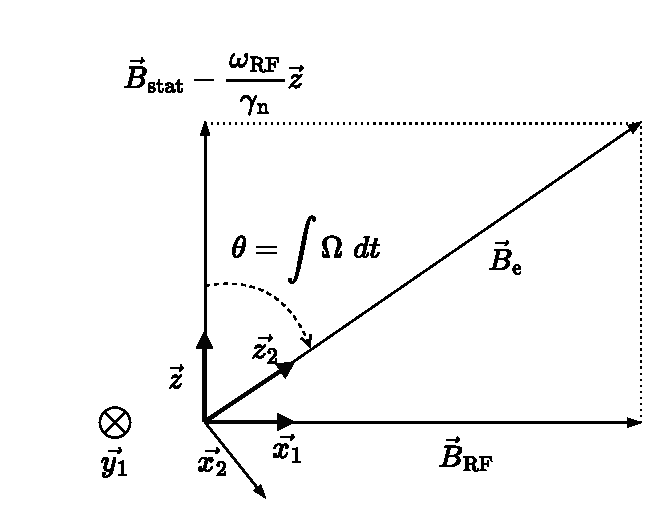
\includegraphics[width=0.5\textwidth]{adiabatic_spin_flip.pdf}
    \caption[{Magnetic fields viewed in the frame of the neutron $\mathcal{R}_1$, which rotates at frequency $\omega_\text{RF}$ about $\vec{z}$}]
            {Magnetic fields viewed in the frame of the neutron $\mathcal{R}_1$, which rotates at frequency $\omega_\text{RF}$ about $\vv{z}$. $\vv{z}=\vv{z_1}$ and $\vv{y_1}=\vv{y_2}$}
    \label{fig:adiabatic_spin_flip}
\end{figure}

A fast adiabatic spin flipper (\acrshort{afp}) is used in the \acrshort*{lanl} \acrshort*{nedm} to provide the option of spin flipping \ucn before the spin analyzer and detector \cite{holley_afp_2012}. The \acrshort*{afp} spin flipper offers the benefit of spin flipping \ucn over a wide velocity range when adiabaticity conditions are satisfied. In this section, we reproduce the spin flip probability derivation from Refs.~\cite{robiscoe_spin_flip, grigoriev_neutron_2001, rogel_thesis}.

An \acrshort*{afp} spin flip requires two magnetic fields: (1)~A static field $\vv{B_\text{stat}}$ in the $\vv{z}$ direction with decreasing strength along $\vv{x}$, and (2)~an oscillating \acrshort{rf} field $\vv{B_\text{RF}}$ with frequency $\omega_\text{RF}$ perpendicular to $\vv{B_\text{stat}}$. Let $\vv{z}$ be the vertical direction, let $\vv{x}$ be the direction the neutron moves through the \acrshort*{afp} region at a velocity $v$, and let time $t=x/v$.

We first change from the lab frame $\mathcal{R}_0(\vv{x},\vv{y}, \vv{z})$ to a frame $\mathcal{R}_1(\vv{x_1},\vv{y_1}, \vv{z_1})$ moving with the neutron while also rotating about $\vv{z}$ at frequency $\omega_\text{RF}$ (see Fig.~\ref{fig:adiabatic_spin_flip}). In $\mathcal{R}_1$, the effective field $\vv{B_\text{e}}(t)$ seen by the neutron is given by
%
\begin{gather}
    \vv{B_\text{e}}(t)=\left(B_\text{stat}(t)-\frac{\omega_\text{RF}}{\gls{gamma_n}}\right)\vv{z}+B_\text{RF}(t)\vv{x} \label{eq:adiab_derivation_1}
\end{gather}
%
where in $\mathcal{R}_1$ we write $\vv{B_\text{RF}}=B_\text{RF}(t)\vv{x_1}$. The frame $\mathcal{R}_1$ is chosen such that:
%
\begin{enumerate}
    \item The static field term $\vv{B_\text{stat}}(t)$ gains a ficticious force field term, $-\omega_\text{RF}/\gls{gamma_n}$ that arises from acceleration due to the rotation of the coordinate frame. At the resonance condition, $\vv{B_\text{stat}} = \vv{B_\text{RF}}$, the first two terms of Eq.~(\ref{eq:adiab_derivation_1}) cancel
    \item $\vv{B_\text{RF}}$ is no longer oscillating
    \item The neutron spin $\vv{S}(t)$ begins precession about $\vv{B_\text{RF}}$ (and effectively begins to follow $\vv{B_\text{e}}$ adiabatically)
\end{enumerate}
%
In the $\mathcal{R}_1$ frame, the Hamiltonian operator $\hat{H}$ with neutron magnetic moment operator $\hat{\gls{mu_n}}$ is
%
\begin{align}
    \hat{H} &= -\hat{\gls{mu_n}}\cdot\vv{B_{e}}=-\gls{gamma_n}\hat{S}\cdot\vv{B_{e}} \nonumber \\
    &= -\gls{gamma_n}\frac{\hbar}{2}\vv{\sigma}\cdot\vv{B_{e}}
\end{align}
%
Referring to Fig.~\ref{fig:adiabatic_spin_flip}, $\vv{B_\text{e}}(t)$ makes an angle $\theta(t)$ with the $\vv{z}$ axis. Therefore,
%
\begin{align}
    \vv{B_\text{e}}(t) &= B_\text{e}(t)\big(\sin\,\theta(t),\,0,\,\cos\,\theta(t) \big) \\
    \Rightarrow \hat{H} &= -\gls{gamma_n}\frac{\hbar}{2}B_{e}(t)\left[\left(\begin{matrix}
                0 & \sin \, \theta(t)\\
                \sin \, \theta(t) & 0
                \end{matrix}\right)+0+\left(\begin{matrix}
                \cos \, \theta(t) & 0\\
                0 & -\cos \, \theta(t)
                \end{matrix}\right)\right] \nonumber \\
    &= -\gls{gamma_n} \frac{\hbar}{2}B_{e}(t)\left(\begin{matrix}
                \cos \, \theta(t) & \sin \, \theta(t)\\
                \sin \, \theta(t) & -\cos \, \theta(t)
                \end{matrix}\right) \label{eq:adiab_derivation_2}
\end{align}
%
Writing the spinor as
$\Ket{\psi(t)}=\Ket{\begin{matrix}
    \psi_{+}(t)\\
    \psi_{-}(t)
\end{matrix}}$ and substituting Eq.~(\ref{eq:adiab_derivation_2}) into (\ref{eq:schrodinger}), the \schrodinger equation, gives
%
\begin{gather}
    \left(\begin{matrix}
    \dot{\psi_{+}}\\
    \dot{\psi_{-}}
    \end{matrix}\right)=\frac{i}{2}\gamma B_{e}(t)\left(\begin{matrix}
    \cos\, \theta(t) & \sin\, \theta(t)\\
    \sin\, \theta(t) & -\cos\, \theta(t)
    \end{matrix}\right)\left(\begin{matrix}
    \psi_{+}\\
    \psi_{-}
    \end{matrix}\right) \label{eq:adiab_derivation_3}
\end{gather}
%
Defining $\omega_\text{e}=-\gamma B_\text{e}$ as the precession frequency about $\vv{B_\text{e}}(t)$, we rewrite Eq.~(\ref{eq:adiab_derivation_3}) in the form
%
\begin{gather}
    \frac{d}{dt}\Ket{\psi(t)}=-\frac{i}{2}\omega_\text{e}\hat{M}\Ket{\psi(t)}
    \label{eq:adiab_derivation_4}
\end{gather}
%
We now want to change to the frame centered about the $\vv{z_2}$ axis, where $\vv{B_\text{e}}(t)$. We use the rotation operator on ket space, $\mathcal{D}_y$, to rotate about the $\vv{y_1}$ axis to reach a reference frame we call $\mathcal{R}_2$. From Ref.~\cite{sakurai_quantum}, Eq.~(3.2.44), we have
%
\begin{align}
    \mathcal{D} &= \exp{\frac{-i\vv{\sigma}\hat{n}\phi}{2}}=\cos \, \frac{\phi}{2}
                            -i\vv{\sigma}\hat{n} \sin \, \frac{\phi}{2} \nonumber \\
                &= \left(\begin{matrix}\cos\left(\phi / 2\right)-i\hat{n_{z}}\sin\left(\phi / 2\right) & (-i\hat{n_{x}}-\hat{n_{y}})\sin\left(\phi / 2\right) \\
                (-i\hat{n_{x}}+\hat{n_{y}})\sin\left(\phi / 2\right) & \cos\left(\phi / 2\right)+i\hat{n_{z}}\sin\left(\phi / 2\right)
                \end{matrix}\right) \label{eq:rotation_operator}
\end{align}
%
A rotation about $\vv{y_1}$ with an angle $\theta(t)$ is therefore
%
\begin{align}
    \mathcal{{D}}_{y}=\left(\begin{matrix}
    \cos\left(\theta / 2\right) & -\sin\left(\theta / 2\right)\\
    \sin\left(\theta / 2\right) & \cos\left(\theta / 2\right)
    \end{matrix}\right)
\end{align}
%
Let us change frames to $\mathcal{R}_2$. We use the transformation $\Ket{\psi(t)}=\mathcal{{D}}_{y}\Ket{\psi'(t)}$, where $\psi'(t)$ is the spinor in frame $\mathcal{R}_2$. Recalling Eq.~(\ref{eq:adiab_derivation_4}) and using the chain rule,
%
\begin{align}
    \frac{d}{dt}\Ket{\psi(t)} &= -\frac{i}{2}\omega_\text{e}\hat{M}\Ket{\psi(t)} \nonumber \\
    \mathcal{{D}}_{y}\frac{d}{dt}\Ket{\psi'(t)}+\dot{\mathcal{{D}}_{y}}\Ket{\psi'(t)}&=-\frac{i}{2}\omega_{e}\hat{M}\mathcal{{D}}_{y}\Ket{\psi'(t)} \nonumber \\
    \frac{d}{dt}\Ket{\psi'(t)}&=-\frac{i}{2}\omega_{e}\mathcal{{D}}_{y}^{-1}\hat{M}\mathcal{{D}}_{y}\Ket{\psi'(t)}-\mathcal{{D}}_{y}^{-1}\dot{\mathcal{{D}}_{y}}\Ket{\psi'(t)}
    \label{eq:adiab_derivation_5}
\end{align}
%
In explicit matrix form, (\ref{eq:adiab_derivation_5}) is
\begin{align}
    \left(\begin{matrix}
    \dot{\psi'_{+}}\\
    \dot{\psi'_{-}}
    \end{matrix}\right)= & -\frac{i}{2}\omega_{e}\left(\begin{matrix}
    \cos\,\frac{\theta}{2} & \sin\,\frac{\theta}{2}\\
    -\sin\,\frac{\theta}{2} & \cos\,\frac{\theta}{2}
    \end{matrix}\right)\left(\begin{matrix}
    \cos\theta & \sin\theta\\
    \sin\theta & -\cos\theta
    \end{matrix}\right)\left(\begin{matrix}
    \cos\,\frac{\theta}{2} & -\sin\,\frac{\theta}{2}\\
    \sin\,\frac{\theta}{2} & \cos\,\frac{\theta}{2}
    \end{matrix}\right)\Ket{\psi'(t)} \nonumber \\
     & -\frac{\dot{\theta}}{2}\left(\begin{matrix}
    \cos\,\frac{\theta}{2} & \sin\,\frac{\theta}{2}\\
    -\sin\,\frac{\theta}{2} & \cos\,\frac{\theta}{2}
    \end{matrix}\right)\left(\begin{matrix}
    -\sin\,\frac{\theta}{2} & -\cos\,\frac{\theta}{2}\\
    \cos\,\frac{\theta}{2} & -\sin\,\frac{\theta}{2}
    \end{matrix}\right)\Ket{\psi'(t)} \nonumber \\
    = & -\frac{i}{2}\omega_{e}\left(\begin{matrix}
    1 & 0\\
    0 & -1
    \end{matrix}\right)\left(\begin{matrix}
    \psi'_{+}\\
    \psi'_{-}
    \end{matrix}\right)-\frac{\dot{\theta}}{2}\left(\begin{matrix}
    0 & -1\\
    1 & 0
    \end{matrix}\right)\left(\begin{matrix}
    \psi'_{+}\\
    \psi'_{-}
    \end{matrix}\right) \label{eq:adiab_derivation_6}
\end{align}
%
We are now in the frame $\mathcal{R}_2$, which follows $\vv{B_\text{e}}(t)$. Let us follow the motion of the neutron spin vector in this frame. Let the total angle of spin precession be $\lambda(t)=\int_0^t\omega_\text{e}(\tau)d\tau$. Again referring to Eq.~(\ref{eq:rotation_operator}), we now want a rotation of angle $\lambda(t)$ about axis $\vv{z_2}$. Let us call this frame $\mathcal{R}_3$. The rotation operator is
%
\begin{gather}
    \mathcal{{D}}_{z2}=\left(\begin{matrix}
    \cos\,\frac{\lambda}{2}-i\sin\,\frac{\lambda}{2} & 0\\
    0 & \cos\,\frac{\lambda}{2}+i\sin\,\frac{\lambda}{2}
    \end{matrix}\right)
    =\left(\begin{matrix}
    e^{-\frac{i}{2}\lambda} & 0\\
    0 & e^{\frac{i}{2}\lambda}
    \end{matrix}\right)
\end{gather}
%
Using the chain rule and the transformation $\Ket{\psi'(t)}=\mathcal{{D}}_{z2}\Ket{\psi''(t)}$
%
\begin{gather}
    \frac{d}{dt}\Ket{\psi''(t)}=\mathcal{{D}}_{z2}^{-1}\left(\frac{d}{dt}\Ket{\psi'(t)}\right)-\mathcal{{D}}_{z2}^{-1}\dot{\mathcal{{D}}_{z2}}\Ket{\psi''(t)}
    \label{eq:adiab_derivation_7}
\end{gather}
%
Here, we know $\frac{d}{dt}\Ket{\psi'(t)}$ from Eq.~(\ref{eq:adiab_derivation_6}). Substituting into Eq.~(\ref{eq:adiab_derivation_7}) gives
%
\begin{align}
    \frac{d}{dt}\Ket{\psi''(t)}= & \mathcal{{D}}_{z2}^{-1}\left[-\frac{i}{2}\omega_{e}\left(\begin{matrix}
    1 & 0\\
    0 & -1
    \end{matrix}\right)\left(\begin{matrix}
    \psi'_{+}\\
    \psi'_{-}
    \end{matrix}\right)-\frac{\dot{\theta}}{2}\left(\begin{matrix}
    0 & -1\\
    1 & 0
    \end{matrix}\right)\left(\begin{matrix}
    \psi'_{+}\\
    \psi'_{-}
    \end{matrix}\right)\right] \nonumber \\
     & -\mathcal{{D}}_{z2}^{-1}\dot{\mathcal{{D}}_{z2}}\Ket{\psi''(t)}
     \label{eq:adiab_derivation_8}
\end{align}
%
where
%
\begin{gather}
    \mathcal{{D}}_{z2}^{-1}=\left(\begin{matrix}
    e^{\frac{i}{2}\lambda} & 0\\
    0 & e^{-\frac{i}{2}\lambda}
    \end{matrix}\right),\quad\dot{\mathcal{{D}}_{z2}}=\frac{\dot{\lambda}}{2}\left(\begin{matrix}
    -ie^{-\frac{i}{2}\lambda} & 0\\
    0 & ie^{\frac{i}{2}\lambda}
    \end{matrix}\right),\nonumber\\
    \text{ and} \quad \mathcal{{D}}_{z2}^{-1}\dot{\mathcal{{D}}_{z2}}=\frac{i\dot{\lambda}}{2}\left(\begin{matrix}
    -1 & 0\\
    0 & 1
    \end{matrix}\right).\nonumber
\end{gather}
%
Observing that $\dot{\lambda}=\omega_\text{e}$ and $\Ket{\psi'(t)}=\mathcal{{D}}_{z2}\Ket{\psi''(t)}$, the first and third terms of Eq.~(\ref{eq:adiab_derivation_8}) cancel out. This leaves
%
\begin{gather}
    \frac{d}{dt}\Ket{\psi''(t)}=\frac{\dot{\theta}}{2}\left(\begin{matrix}
    0 & e^{\frac{i}{2}\lambda}\\
    -e^{-\frac{i}{2}\lambda} & 0
    \end{matrix}\right)\left(\begin{matrix}
    \psi'_{+}\\
    \psi'_{-}
    \end{matrix}\right)\label{eq:adiab_derivation_9}
\end{gather}
%
To solve for Eq.~(\ref{eq:adiab_derivation_9}), we must change to $\theta$ as the independent variable. $\lambda$ becomes a function of $\theta$ by the adiabatic parameter \gls{adiab} introduced in Sec.~\ref{sec:adiabaticity}. 
%
\begin{gather}
\lambda =\int_{0}^{t}\omega_{e}(\tau)d\tau
 =\int_{0}^{\theta}\frac{\omega_{e}}{\dot{\theta}}d\theta
 =\int_{0}^{\theta}\gls*{adiab}(\theta)d\theta
 \label{eq:adiab_derivation_10}
\end{gather}
%
where we used the relations $\dot{\theta}=d\theta/d\tau,\,\,\gls*{adiab}(t)=\left|\omega_\text{e}/\Omega(t)\right|,$ and let the rotation rate of $\vv{B_\text{e}}(t)$ be $\Omega(t)=\dot{\theta}$. Eq.~(\ref{eq:adiab_derivation_9}) becomes
%
\begin{align}
\frac{d\psi''_{+}}{d\theta}= & \frac{1}{2}e^{-\lambda}\psi''_{-}
\label{eq:adiab_derivation_11}\\
\frac{d\psi''_{-}}{d\theta}= & -\frac{1}{2}e^{-i\lambda}\psi''_{+}
\label{eq:adiab_derivation_12}
\end{align}
%
To decouple, we take another derivative with respect to $\theta$ to obtain $d^2\psi''_{+}/d\theta^2$ and $d^2\psi''_{-}/d\theta^2$. Then we use $\dot{\lambda}=\gls*{adiab}(\theta)$, (\ref{eq:adiab_derivation_11}), and (\ref{eq:adiab_derivation_12}) to obtain the last set of equations that need to be solved,
%
\begin{align}
\frac{d^{2}\psi''_{+}}{d\theta^{2}}-i\gls*{adiab}\frac{d\psi''_{+}}{d\theta}+\frac{1}{4}\psi''_{+} & =0\\
\frac{d^{2}\psi''_{-}}{d\theta^{2}}+i\gls*{adiab}\frac{d\psi''_{-}}{d\theta}+\frac{1}{4}\psi''_{-} & =0
\end{align}
%
which, for constant \gls{adiab}, has a solution of the form
%
\begin{gather}
    \psi''_\pm=\exp\left( \pm \frac{i\gls*{adiab}\theta}{2} \right)
                \left[C_{\psi\pm}\cos \left(\frac{\theta}{2}\sqrt{1+\gls*{adiab}^2} \right)  
                + i D_{\psi\pm}\sin \left(\frac{\theta}{2}\sqrt{1+\gls*{adiab}^2} \right)
                \right]
\end{gather}
%
At time $t=0$, we have $\theta=0$, and the neutron is in an initial unflipped state $\psi_+=1,\,\,\psi_-=0$. To translate these initial conditions from $\mathcal{{R}}_{1}\rightarrow\mathcal{{R}}_{3}$, from our rotation operators we have
%
\begin{gather}   
    \Ket{\psi(t)}=\mathcal{{D}}_{y}\Ket{\psi'(t)}=\mathcal{{D}}_{y}\mathcal{{D}}_{z2}\Ket{\psi''(t)} \\
    \Rightarrow\Ket{\psi''(t)}=\mathcal{{D}}_{z2}^{-1}\mathcal{{D}}_{y}^{-1}\Ket{\psi(t)}
    \label{eq:adiab_derivation_13}
\end{gather}
%
Solving for initial conditions gives
%
\begin{align}
    \psi''_{+} &= e^{\frac{i\gls*{adiab}\theta}{2}}\left(\cos\left(\frac{\theta}{2}\sqrt{1+\gls*{adiab}^{2}}\right)-\frac{i\gls*{adiab}}{\sqrt{1+\gls*{adiab}^{2}}}\sin\left(\frac{\theta}{2}\sqrt{1+\gls*{adiab}^{2}}\right)\right) 
    \label{eq:adiab_derivation_14}\\
    \psi''_{-} &= -\frac{\exp\left(-\frac{i\gls*{adiab}\theta}{2}\right)}{\sqrt{1+\gls*{adiab}^{2}}}\sin\left(\frac{\theta}{2}\sqrt{1+\gls*{adiab}^{2}}\right)
    \label{eq:adiab_derivation_15}
\end{align}
%
Finally, using (\ref{eq:adiab_derivation_13}), (\ref{eq:adiab_derivation_14}), and (\ref{eq:adiab_derivation_15}) to obtain $\Ket{\psi}$, and examining when the field $\vv{B_\text{e}}$ has turned by $\pi$ radians,
%
\begin{align}
    |\psi_{+}|^{2} &= \frac{1}{1+\gls*{adiab}^{2}}\sin^{2}\left(\frac{\pi}{2}\sqrt{1+\gls*{adiab}^{2}}\right) \\
    |\psi_{-}|^{2} &= 1-|\psi_{+}|^{2} \label{eq:adiab_derivation_16}
\end{align}
%
In this section the adiabaticity parameter is written in terms of precession about the effective field $\vv{B_\text{e}}$ and the rotation rate of the effective field 
%
\begin{gather}
    \gls*{adiab}(t)=\left|\frac{\omega_\text{e}}{\Omega(t)}\right| \label{eq:adiab_AFP}
\end{gather}
%
This differs slightly from the version introduced in Sec.~\ref{sec:adiabaticity}, which is written in terms of a more general local field. Let us write a more practical definition for spin flipper adiabaticity. For the amplitude of the \acrshort*{rf} field along the neutron path $x=[0,\ell_0]$, we can write the form \cite{grigoriev_neutron_2001}
%
\begin{gather}
    B_\text{RF}=A\sin \left(\pi \frac{x}{\ell_0}\right) = A\sin \left(\pi \frac{vt}{\ell_0}\right)\label{eq:adiab_derivation_17}
\end{gather}
%
$A$ is the modulation amplitude and $\ell_0$ is the the length of the flipper. We let $B_0$ be the field in the center of the flipper $x_0=\ell_0/2$, so that we may write the static field amplitude as
%
\begin{gather}
    B_\text{stat}=B_0 + A\cos\left(\pi \frac{x}{\ell_0}\right) =B_0 + A\cos\left(\pi \frac{vt}{\ell_0}\right)\label{eq:adiab_derivation_18}
\end{gather}
%
The second term of Eq.~(\ref{eq:adiab_derivation_18}) manifests as a permanent gradient field superimposed onto a uniform field $B_0$. From Fig.~\ref{fig:adiabatic_spin_flip}, we also have
%
\begin{gather}
    B_\text{e}=\sqrt{B_\text{RF}^2+\left(B_\text{stat}-\frac{\omega_\text{RF}}{\gls*{gamma_n}} \right)^2}
\end{gather}
%
Again referring to Fig.~\ref{fig:adiabatic_spin_flip}, we find $\Omega$ to be
%
\begin{align}
    \Omega(t) &= \frac{d\theta}{dt}= \frac{d}{dt}\left( \arcsin \frac{B_\text{RF}}{B_\text{e}} \right) = 
    \frac{B_\text{e}\dot{B}_\text{RF}-B_\text{RF}\dot{B}_\text{e}}
    {B_\text{e}^2\sqrt{1-(B_\text{RF}/B_\text{e})^2}} \\
    &\approx \frac{\left(B_\text{stat}-\frac{\omega_\text{rf}}{\gls*{gamma_n}} \right)\dot{B}_\text{RF}-B_\text{RF}\dot{B}_\text{stat}}
    {B_\text{e}^2}
     \label{eq:adiab_derivation_19}
\end{align}
%
At the resonant point, we have $t_0=\ell_0/(2v)$ and $B_0=\omega_\text{RF}/\gls*{gamma_n}$. Therefore, using Eqs.~(\ref{eq:adiab_derivation_17}), (\ref{eq:adiab_derivation_18}), and (\ref{eq:adiab_derivation_19}), Eq.~(\ref{eq:adiab_AFP}) becomes
%
\begin{gather}
    \gls*{adiab} = \frac{\gls*{gamma_n} \ell_0 A}{\pi v}
\end{gather}
%
Eq.~(\ref{eq:adiab_derivation_16}) gives the chance of measuring a different spin state after the neutron has passed through the spin flipper region (i.e., $\vv{S}$ has followed $\vv{B_\text{e}}$ adiabatically). For constant \gls*{adiab}, the spin flip probability is
%
\begin{gather}
    P=1-\frac{1}{1+\gls*{adiab}^{2}}\sin^{2}\left(\frac{\pi}{2}\sqrt{1+\gls*{adiab}^{2}}\right)
\end{gather}


\comment{TODO: Plot evolution of probability as a function of \gls*{adiab} (see Pierre thesis pg 53)}

